\section{Методы классификации биосигналов}
\label{sec:Chapter2}

В~данном разделе описываются три модели машинного обучения,
реализованные в~работе, а~также метод вейвлет-анализа,
применявшийся для~частотно-временного исследования ЭКГ-сигналов.

\subsection{Случайный лес}

\subsubsection{Алгоритм}

Случайный лес~(Random Forest)~\cite{breiman2001}~--- ансамблевый
метод, основанный на~бэггинге над~деревьями решений.
Для~задачи классификации с~$T$ деревьями ответ модели определяется
голосованием большинства:
\begin{equation}
    \hat{y} = \operatorname*{arg\,max}_{k \in \mathcal{Y}}
    \sum_{t=1}^{T} \mathbf{1}[\,h_t(\mathbf{x}) = k\,],
\end{equation}
где $h_t(\mathbf{x})$~--- предсказание $t$-го дерева.

Каждое дерево обучается на~бутстрэп-выборке из~обучающих данных,
а~при~выборе оптимального разбиения в~каждом узле рассматривается
случайное подмножество $m \approx \sqrt{d}$ признаков.
Такая рандомизация снижает корреляцию между деревьями и~уменьшает
дисперсию ансамбля~\cite{breiman2001}.

\subsubsection{Настройка гиперпараметров}

В~работе используется $T = 200$ деревьев.
Для~компенсации дисбаланса классов применяется стратегия
\texttt{balanced\_subsample}: при~формировании каждого
бутстрэп-экземпляра производится стратифицированная
ресамплировка, обеспечивающая равное число объектов каждого
класса в~обучающей порции дерева.
Функционал информативности узла~--- критерий Джини.

\subsubsection{Важность признаков}

Случайный лес позволяет оценить вклад каждого признака $j$
в~качество классификации через среднее уменьшение примеси~(MDI):
\begin{equation}
    \mathrm{Imp}(j) = \frac{1}{T}\sum_{t=1}^{T}
    \sum_{\text{узлы с разб.\ по }j}
    \Delta\mathrm{Gini}_t \cdot \frac{n_\text{узел}}{n},
\end{equation}
где $\Delta\mathrm{Gini}_t$~--- уменьшение индекса Джини в~узле.
Анализ важности признаков позволяет интерпретировать, какие
временны\'{е} участки кардиоцикла наиболее информативны
при~разделении классов.

\subsection{Одномерная сверточная нейронная сеть (1D CNN)}

\subsubsection{Мотивация}

Сверточные нейронные сети~\cite{lecun1998} обладают свойством
\textit{трансляционной инвариантности}: один и~тот~же паттерн
формы QRS-комплекса обнаруживается вне~зависимости от~его
положения в~окне.
Применение одномерных сверток к~временному ряду ЭКГ позволяет
автоматически извлекать иерархические признаки: от~низкоуровневых
перепадов амплитуды до~высокоуровневых форм зубцов.

\subsubsection{Архитектура}

Входной тензор имеет форму $(\text{batch},\,1,\,240)$~---
один канал, $240$ временны\'{х} отсчетов.
Сеть состоит из~\textit{сверточного} блока и~\textit{классификатора}
(таблица~\ref{tab:cnn_arch}).

\begin{table}[h]
\centering
\caption{Архитектура 1D~CNN}
\label{tab:cnn_arch}
\begin{tabular}{llrr}
\hline
\textbf{Слой} & \textbf{Параметры} &
\textbf{Выход $(C \times L)$} & \textbf{Параметры, шт.} \\
\hline
Conv1d       & $1\to16$, $k=7$, $p=3$ & $16\times240$ & 128  \\
BatchNorm1d  & $16$                   & $16\times240$ & 32   \\
ReLU         & ---                    & $16\times240$ & 0    \\
MaxPool1d    & $k=2$                  & $16\times120$ & 0    \\
\hline
Conv1d       & $16\to32$, $k=5$, $p=2$ & $32\times120$ & 2\,592 \\
BatchNorm1d  & $32$                    & $32\times120$ & 64    \\
ReLU         & ---                     & $32\times120$ & 0     \\
MaxPool1d    & $k=2$                   & $32\times60$  & 0     \\
\hline
Conv1d       & $32\to64$, $k=5$, $p=2$ & $64\times60$ & 10\,304 \\
BatchNorm1d  & $64$                     & $64\times60$ & 128     \\
ReLU         & ---                      & $64\times60$ & 0       \\
MaxPool1d    & $k=2$                    & $64\times30$ & 0       \\
\hline
Flatten      & ---                      & $1920$       & 0       \\
Linear       & $1920\to128$             & $128$        & 245\,888 \\
ReLU         & ---                      & $128$        & 0        \\
Dropout      & $p=0.3$                  & $128$        & 0        \\
Linear       & $128\to5$                & $5$          & 645      \\
\hline
\multicolumn{3}{l}{\textbf{Итого обучаемых параметров}} & \textbf{259\,781} \\
\hline
\end{tabular}
\end{table}

Три стадии свертки с~попарным пулингом уменьшают длину
временного ряда с~$240$ до~$30$ отсчетов, одновременно
увеличивая число карт признаков с~$1$ до~$64$.
Регуляризация достигается через~BatchNorm после~каждой свертки
и~Dropout ($p=0.3$) перед выходным слоем.

\subsubsection{Обучение}

Оптимизатор~--- Adam~\cite{kingma2014} с~начальной скоростью обучения
$\eta_0 = 10^{-3}$.
Планировщик ReduceLROnPlateau снижает $\eta$ вдвое, если Macro~F1
на~валидации не~улучшается в~течение $3$~эпох:
$\eta \leftarrow 0.5\,\eta$.
Ранняя остановка с~patience~$=5$ предотвращает переобучение.
Число эпох~--- не~более~$20$; наилучшие веса по~Macro~F1 сохраняются
отдельно.

\subsection{Остаточная нейронная сеть (ResNet1D)}

\subsubsection{Мотивация и остаточное соединение}

При~увеличении глубины нейронной сети возникает проблема
затухающих градиентов: сигнал ошибки, распространяясь в~обратном
направлении, многократно умножается на~небольшие числа и~«исчезает»
в~ранних слоях~\cite{goodfellow2016}.
He~и~др.~\cite{he2016} предложили архитектуру с~\textit{остаточными
соединениями} (skip connections), вычисляющую не~прямое
отображение $H(\mathbf{x})$, а~остаток $F(\mathbf{x})$:
\begin{equation}
    \label{eq:residual}
    \mathbf{y} = F(\mathbf{x},\,\{W_i\}) + \mathbf{x},
\end{equation}
где $F(\mathbf{x})$~--- нелинейное преобразование двух сверточных
слоев, а~$\mathbf{x}$~--- прямая «шунтирующая» ветвь.
Такое соединение устраняет проблему затухания и~позволяет
обучать существенно более глубокие сети.

\subsubsection{Архитектура}

Реализованная модель ResNet1D состоит из~начального стволового
слоя (\textit{stem}) и~трех остаточных блоков
(таблица~\ref{tab:resnet_arch}).

\begin{table}[h]
\centering
\caption{Архитектура ResNet1D}
\label{tab:resnet_arch}
\begin{tabular}{lllr}
\hline
\textbf{Блок} & \textbf{Состав} & \textbf{Выход $(C \times L)$} &
\textbf{stride} \\
\hline
Stem     & Conv1d($1\to16$, $k=7$) + BN + ReLU & $16\times240$ & 1 \\
\hline
Layer\,1 & ResidualBlock($16\to16$, $k=7$)     & $16\times240$ & 1 \\
Layer\,2 & ResidualBlock($16\to32$, $k=7$)     & $32\times120$ & 2 \\
Layer\,3 & ResidualBlock($32\to64$, $k=7$)     & $64\times60$  & 2 \\
\hline
Pool     & AdaptiveAvgPool1d(1)                 & $64\times1$   & --- \\
FC       & Linear($64\to5$)                    & $5$           & --- \\
\hline
\end{tabular}
\end{table}

Каждый \textit{ResidualBlock} содержит две последовательные
свертки с~BatchNorm и~ReLU, а~также адаптивный шунт:
если размерности входа и~выхода не~совпадают (по~каналам или
длине), шунт реализуется сверткой $1\times1$ со~stride; иначе~---
тождественным отображением (Identity).
После сложения $F(\mathbf{x}) + \text{shortcut}(\mathbf{x})$
применяется ReLU.

Слой \texttt{AdaptiveAvgPool1d(1)} глобально усредняет
карту признаков по~временному измерению, что~делает сеть
нечувствительной к~его абсолютной длине.
Итоговый вектор из~$64$ нейронов подается в~линейный
классификатор.

\subsubsection{Обучение}

Конфигурация обучения аналогична CNN: оптимизатор Adam
($\eta_0 = 10^{-3}$), взвешенная кросс-энтропия
(формулы~\eqref{eq:weights},~\eqref{eq:wce}),
ReduceLROnPlateau~($\times0.5$, patience~$=3$),
ранняя остановка (patience~$=7$), не~более~$30$~эпох.
Перед обучением признаки нормализуются по~формуле~\eqref{eq:scaler},
параметры нормализации сохраняются для~последующей оценки.

\subsection{Вейвлет-анализ ЭКГ-сигналов}

\subsubsection{Ограничения преобразования Фурье}

Классическое преобразование Фурье дает полную информацию
о~частотном составе сигнала, но~не~позволяет установить,
\textit{в~какой момент времени} та~или~иная частота присутствует.
Поскольку ЭКГ является нестационарным сигналом~--- его
характеристики меняются на~протяжении одного кардиоцикла
(зубцы~P, QRS, T имеют различные частотные составы)~---
для~его анализа требуется инструмент совместного
частотно-временного представления~\cite{zakharova2018}.

\subsubsection{Дискретное вейвлет-преобразование}

Дискретное вейвлет-преобразование~(ДВП) разлагает сигнал
$s[n]$ по~ортонормированному базису масштабирующих функций
и~вейвлетов методом пирамидального алгоритма Малла~\cite{mallat1989}.
На~каждом уровне разложения $j$ сигнал пропускается
через пару фильтров: фильтр нижних частот дает
коэффициенты приближения~$\{a_j[n]\}$, фильтр верхних частот~---
коэффициенты детализации~$\{d_j[n]\}$:
\begin{equation}
    a_j[n] = \sum_k h[k]\, a_{j-1}[2n-k], \quad
    d_j[n] = \sum_k g[k]\, a_{j-1}[2n-k],
\end{equation}
где $h[k]$ и~$g[k]$~--- коэффициенты квадратурных зеркальных
фильтров, определяемых выбором вейвлета.

В~работе используется вейвлет Добеши~4 (db4), обладающий
$4$~нулевыми моментами~--- что~обеспечивает компактную
запись гладких сигналов~--- и~хорошо согласованный
с~формой QRS-комплекса~\cite{zakharova2018}.
При~$L = 4$ уровнях разложения и~частоте дискретизации
$f_s = 360$~Гц формируются следующие частотные подполосы
(таблица~\ref{tab:wavelet_bands}).

\begin{table}[h]
\centering
\caption{Частотные подполосы ДВП db4 при $f_s = 360$~Гц}
\label{tab:wavelet_bands}
\begin{tabular}{clll}
\hline
\textbf{Подполоса} & \textbf{Частоты, Гц} & \textbf{Физ.\ смысл для ЭКГ} &
\textbf{Число коэф.} \\
\hline
$\mathrm{cD}_1$ & $90\text{–}180$ & Высокочастотный шум (ЭМГ) & $\approx 120$ \\
$\mathrm{cD}_2$ & $45\text{–}90$  & Высокочаст.\ компоненты QRS  & $\approx 60$ \\
$\mathrm{cD}_3$ & $22.5\text{–}45$& Комплекс QRS                 & $\approx 30$ \\
$\mathrm{cD}_4$ & $11\text{–}22.5$& Зубцы P и T                  & $\approx 15$ \\
$\mathrm{cA}_4$ & $0\text{–}11$   & Изолиния, дрейф              & $\approx 15$ \\
\hline
\end{tabular}
\end{table}

\subsubsection{Вейвлет-признаки для случайного леса}

Для~расширения векторного представления каждого кардиоцикла
из~коэффициентов каждой подполосы~$\mathrm{cX}_j$ извлекаются
$5$ статистических признаков:
\begin{equation}
    \boldsymbol{\phi}(\mathrm{cX}_j) = \Bigl(
    \bar{c}_j,\;\sigma_j,\;E_j,\;\max|\mathrm{cX}_j|,\;\gamma_{1,j}
    \Bigr),
\end{equation}
где $\bar{c}_j$~--- среднее, $\sigma_j$~--- стандартное отклонение,
$E_j = \mathrm{mean}(\mathrm{cX}_j^2)$~--- энергия,
$\gamma_{1,j}$~--- коэффициент асимметрии.
Таким образом, каждый удар дополнительно описывается вектором
из~$5 \times 5 = 25$ вейвлет-признаков.

В~проведенном эксперименте (раздел~\ref{sec:Chapter3}) добавление
вейвлет-признаков к~$240$~временны\'{м} отсчетам не~улучшило
качество случайного леса: Macro~F1~$= 0.9479$ (с~вейвлетом)
против~$0.9496$ (без~него).
Это объясняется тем, что~ансамбль деревьев неявно обнаруживает
частотно-временны\'{е} паттерны непосредственно из~временного ряда,
тогда как~агрегатные статистики коэффициентов теряют позиционную
информацию.
Тем~не~менее вейвлет-анализ представляет значительную ценность
для~\textit{интерпретации} сигналов: скаллограммы~(рисунок~\ref{fig:cwt})
и~распределение энергии по~подполосам~(рисунок~\ref{fig:wt_energy})
наглядно демонстрируют, как~различные классы аритмий отличаются
в~частотно-временном пространстве.

\begin{figure}[h]
\centering
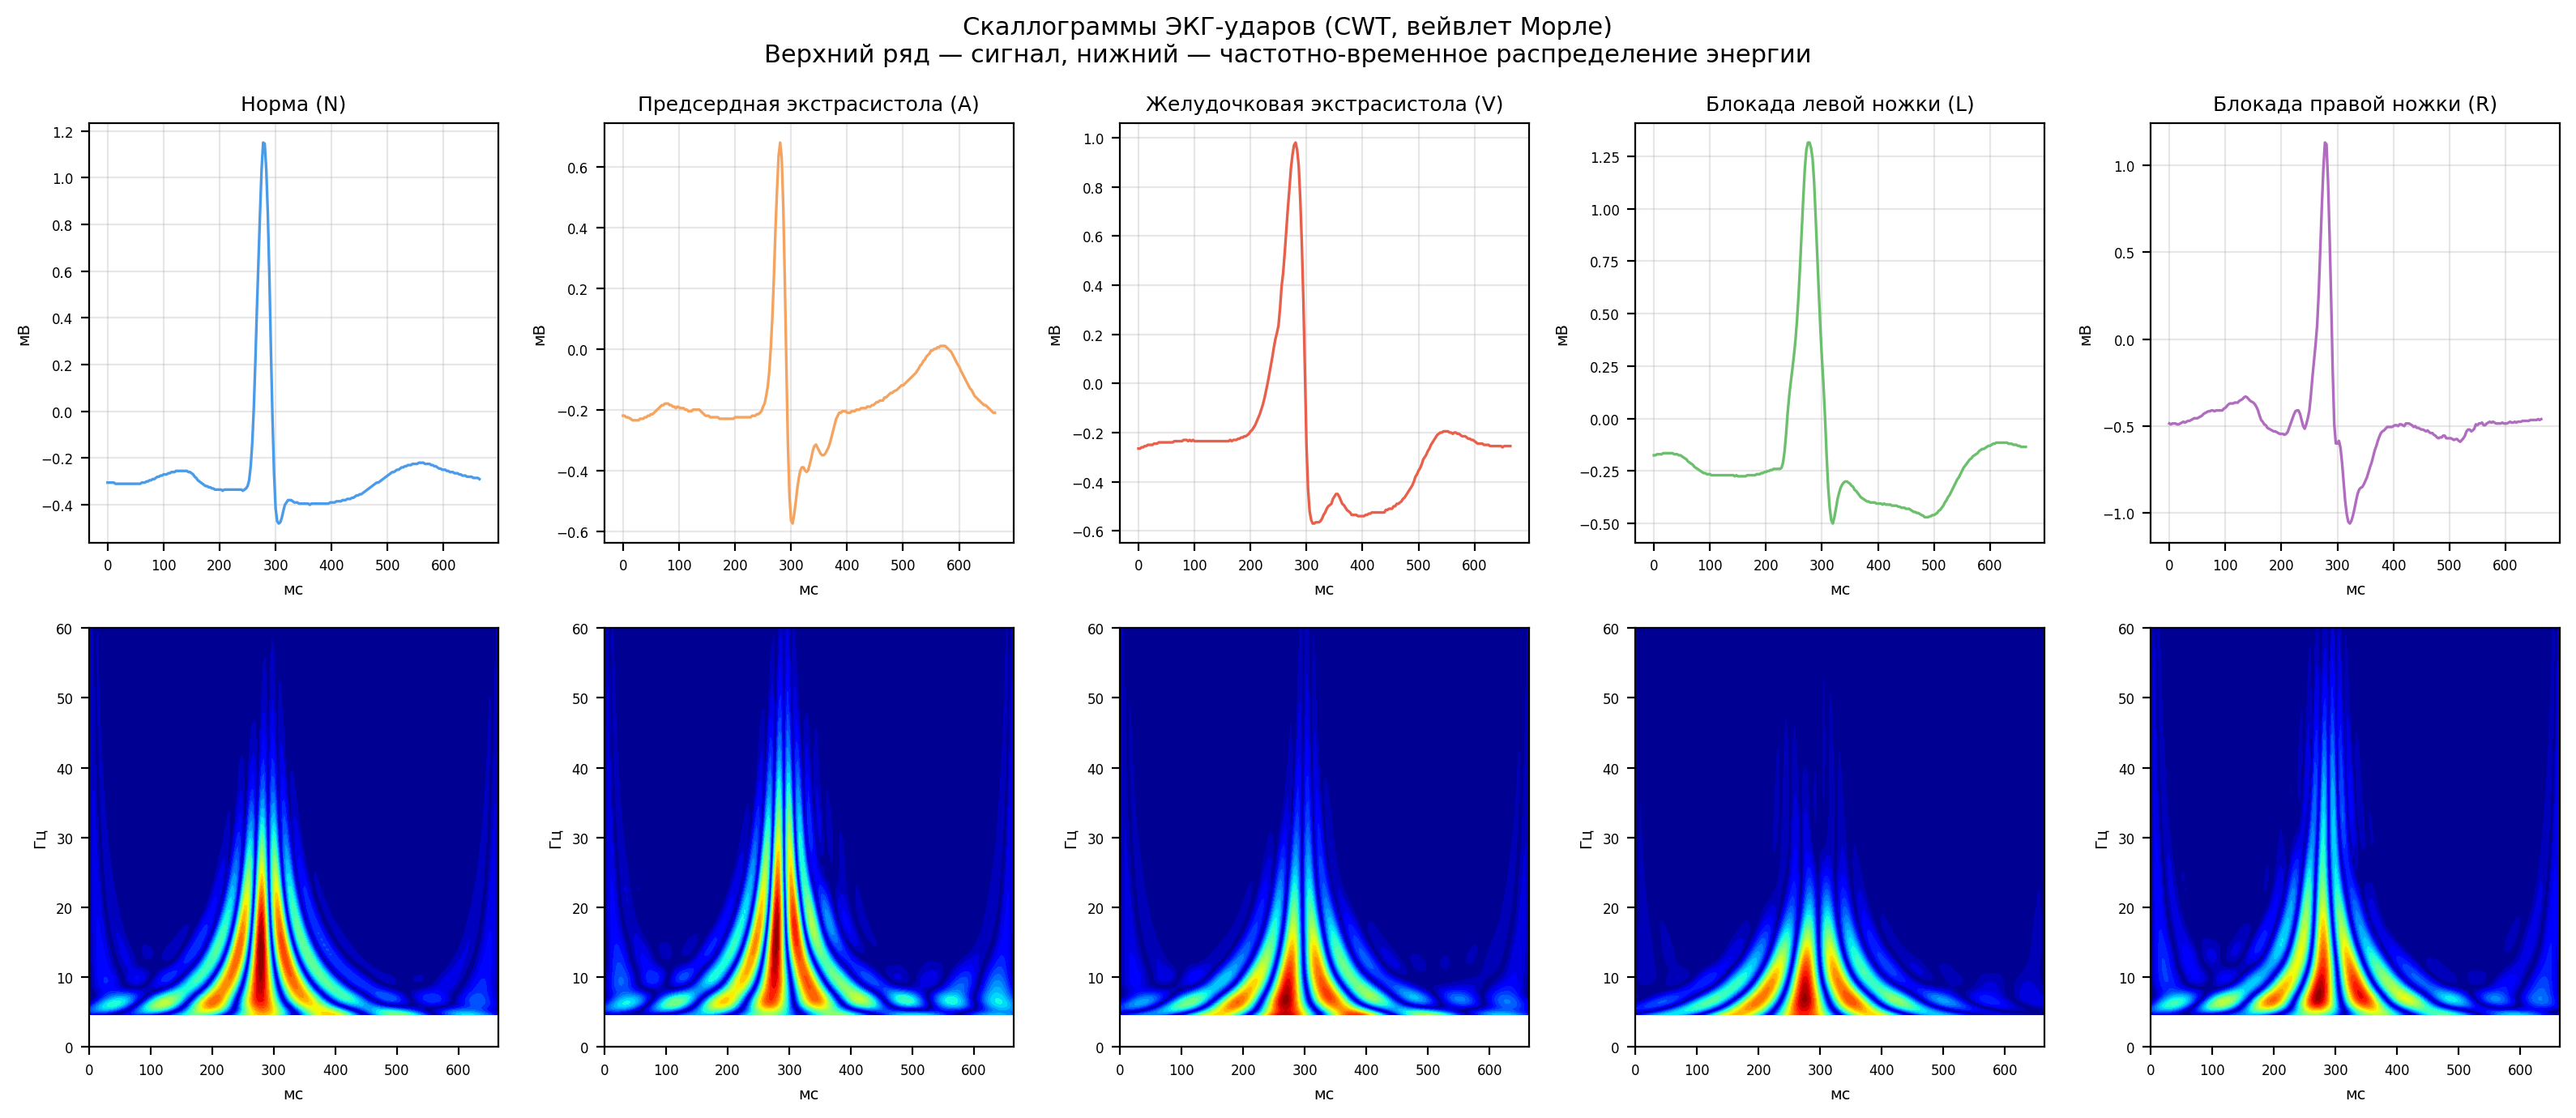
\includegraphics[width=\textwidth]{../reports/figures/models/wavelet_cwt_gallery.png}
\caption{Скаллограммы CWT (вейвлет Морле) для медианного удара каждого класса.
Верхний ряд~--- временной сигнал, нижний~--- частотно-временное распределение
энергии.}
\label{fig:cwt}
\end{figure}

\begin{figure}[h]
\centering
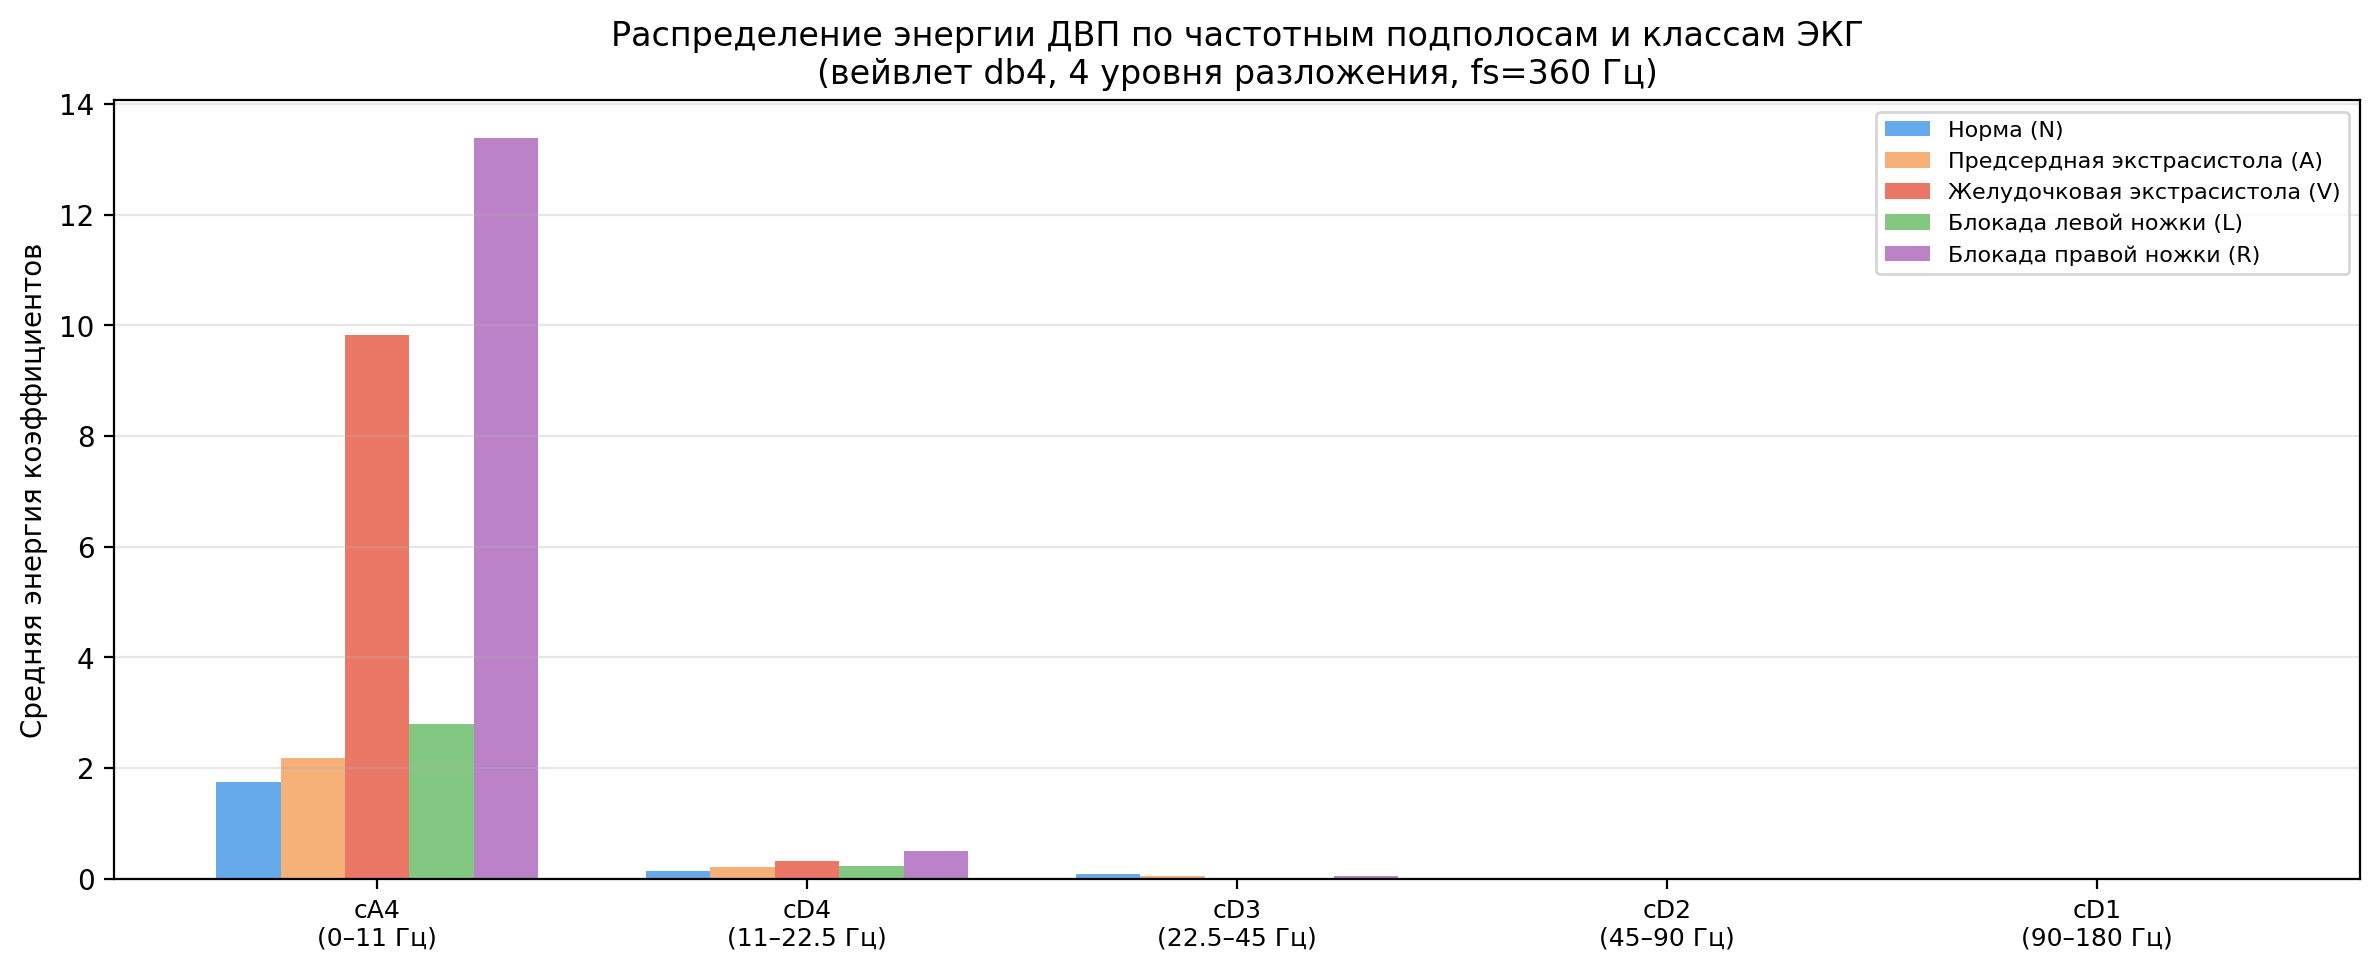
\includegraphics[width=0.95\textwidth]{../reports/figures/models/wavelet_avg_energy.png}
\caption{Средняя энергия коэффициентов ДВП db4 по~частотным подполосам и~классам.
Различие классов~V и~A в~подполосах $\mathrm{cD}_3$--$\mathrm{cD}_4$
отражает разницу в~форме QRS-комплекса.}
\label{fig:wt_energy}
\end{figure}

\subsection{Сравнительный анализ методов}

Три рассматриваемые модели занимают различные позиции
в~пространстве <<точность~--- интерпретируемость~--- устойчивость>>
(таблица~\ref{tab:model_comparison}).

\begin{table}[h]
\centering
\caption{Качественное сравнение моделей}
\label{tab:model_comparison}
\begin{tabular}{lccccc}
\hline
\textbf{Критерий} & \textbf{RF} & \textbf{1D~CNN} & \textbf{ResNet1D} \\
\hline
Интерпретируемость     & Высокая  & Низкая   & Низкая  \\
Нормализация           & Не нужна & Нужна    & Нужна   \\
Устойчивость к~шуму    & Высокая  & Средняя  & Средняя \\
Гиперпараметров        & Мало     & Умеренно & Много   \\
Время обучения         & Быстро   & Умеренно & Медленно \\
Качество (Macro~F1)    & 0.950    & \textbf{0.974}    & 0.953   \\
\hline
\end{tabular}
\end{table}

Случайный лес выигрывает по~простоте настройки и~интерпретируемости.
1D~CNN достигает наилучшего качества классификации за~счет
автоматического извлечения признаков.
ResNet1D потенциально мощнее, но~требует большего числа эпох
для~сходимости и~чувствителен к~инициализации.
